\section{Exercise 7}

Consider the following code: 
\begin{verbnobox}[\verbarg]
#include <stdio.h>
#include <stdlib.h>
#include <string.h>

void encrypt(int backdoor){
    struct{
        char tmp[38];
        char msg[48];
    } e;

    strcpy(e.msg, "*Decrypted*:");
    printf("Insert the message to encrypt here\n");
    scanf("\%38s", e.tmp);
    strncat(e.msg, e.tmp, 48); // concatenate the two strings
    if (backdoor == 1){
        printf(e.msg);
    }else{
        printf("Encrypted: *****************\n");
    }
}

int verify(){
    struct{
        char sec1[8];
        char sec2[16];
        char *p;
    } s;

    s.p = s.sec1;
    s.backdoor = 0;

    printf("Please insert the encryption secret\n");
    scanf ("\%s", s.sec2);
    scanf ("\%7s", s.p);
    if (strncmp(s.sec2, "FL4G", 4) == 0) {
        encrypt(s.backdoor);
        return 1;
    }
    printf("To be, or not to be, that is the question...\n");
    abort ();
}

void main (int argc, char **argv){
    verify();
}
\end{verbnobox}
\begin{enumerate}
    \item The program may be affected by a typical buffer overflow vulnerability. 
        Specify the vulnerable line/s of code. 
        Motivate the answer.
    \item The program may be affected by a typical format string vulnerability. 
        Specify the vulnerable line/s of code. 
        Motivate the answer.
    \item From now on, assume the program is compiled for the x86 architecture (32 bit) and for an environment that adopts the usual cdecl calling convention. 
        Furthermore, assume that no compiler-level or OS-level mitigations against the exploitation of memory corruption errors is present (unless specified otherwise). 
        Draw the stack layout after the program has executed the instruction at line 32, showing:
        \begin{itemize}
            \item Direction of growth and high-low addresses;
            \item The name of each allocated variable;
            \item The content of relevant registers (i.e., EBP, ESP);
            \item The functions stack frames.
        \end{itemize}
        Show also the content of the caller frame.
    \item Focus only on the stack-based buffer overflow vulnerability. 
        Write an exploit for this vulnerability that executes the following shell code, composed of 7 bytes: 
\begin{verbatim}
0x31 0xc0 0x40 0x89 0xc3 0xcd 0x80   
\end{verbatim}
        Make sure that you show how the exploit will appear in the process memory with respect to the stack layout right before and after the execution of the vulnerable line during the program exploitation.
        Ensure you describe all the steps and assumptions required for a successful exploitation of the vulnerability. 
        Include also any assumption on how you must call the program (e.g., the values for the command-line arguments required to trigger the exploit correctly and/or environment variables, if any).
    \item Focus only on the stack-based buffer overflow vulnerability. 
        Assume that the program is compiled only with the correct implementation of the compiler-level mitigation known as “Random Stack Canary” (the address space layout is not randomized, and the stack is executable). 
        Is it effective to prevent your exploit at previous point? 
        If the mitigation technique is effective, explain why and describe how you would modify the buffer overflow exploit to bypass the mitigation.
        If it is not effective, please explain why.
    \item Now focus on the format string vulnerability only. Write an exploit for this vulnerability that executes the previous shell code you have already allocated in memory. 
    Assume that:
    \begin{itemize}
        \item The address of the return address (saved EIP) of the function verify is: 0xffffb5d8 (i.e., where to write).
        \item The address of the first instruction of the shell code is at: 0xf4d0e349 (i.e., what to write).
        \item The displacement on the stack of the vulnerable function's argument is: 2
    \end{itemize}
    Knowing that dec( 0xf4d0) = 62672 and dec(0xe349) = 58185, write the exploit clearly, detailing all the  components of the format string and all the steps that lead to a successful exploitation.
    
\end{enumerate}

\subsection*{Solution}
\begin{enumerate}
    \item There is a buffer overflow ar line 37 because it reads an entire string without considering the length. 
    \item There is a format string at line 16 because it prints a string without a format specifier. 
    \item The stack is composed as follows: 
        \begin{figure}[H]
            \centering
            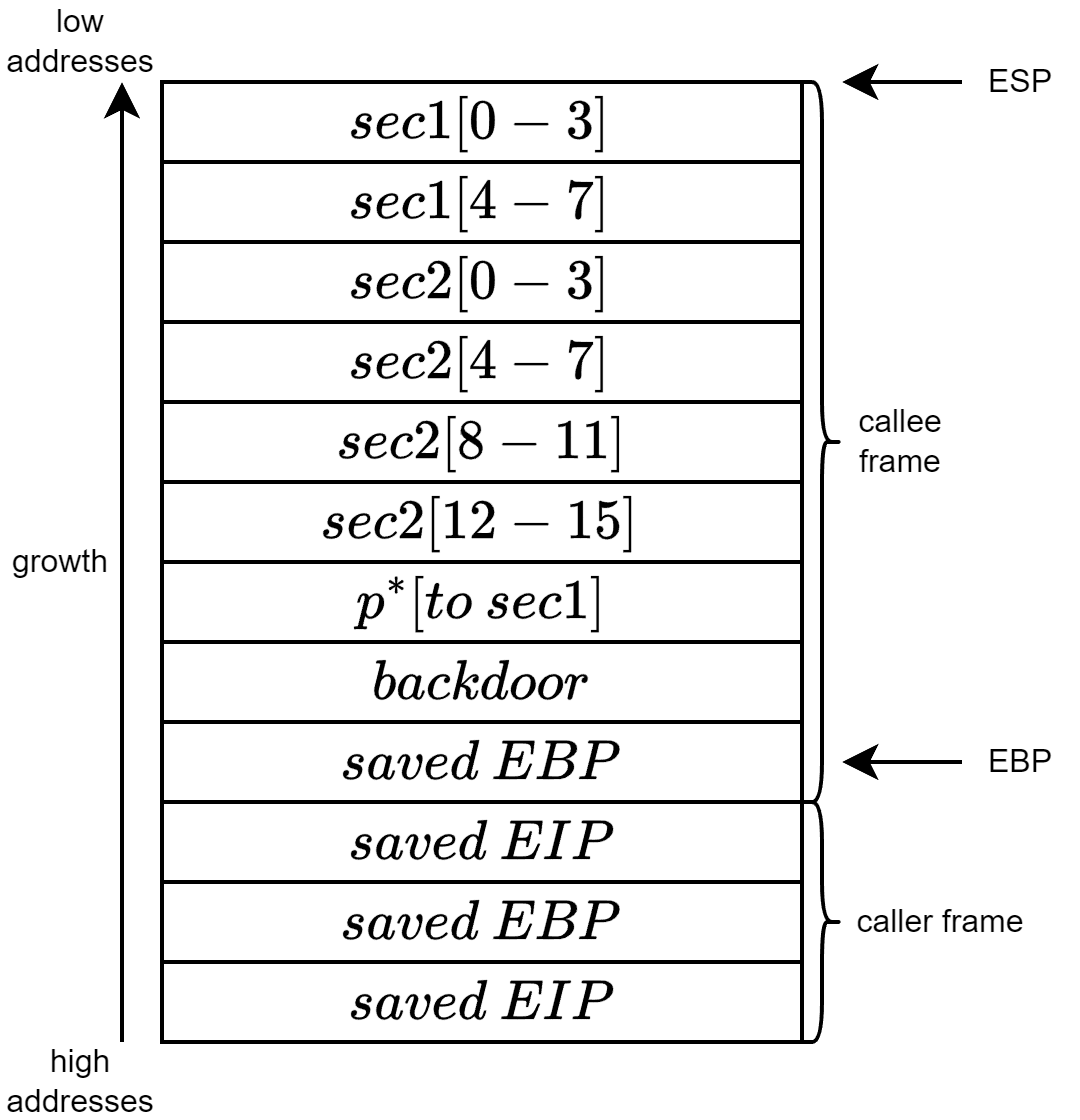
\includegraphics[width=0.5\linewidth]{images/stack10.png}
        \end{figure}
    \item The stack becomes: 
        \begin{figure}[H]
            \centering
            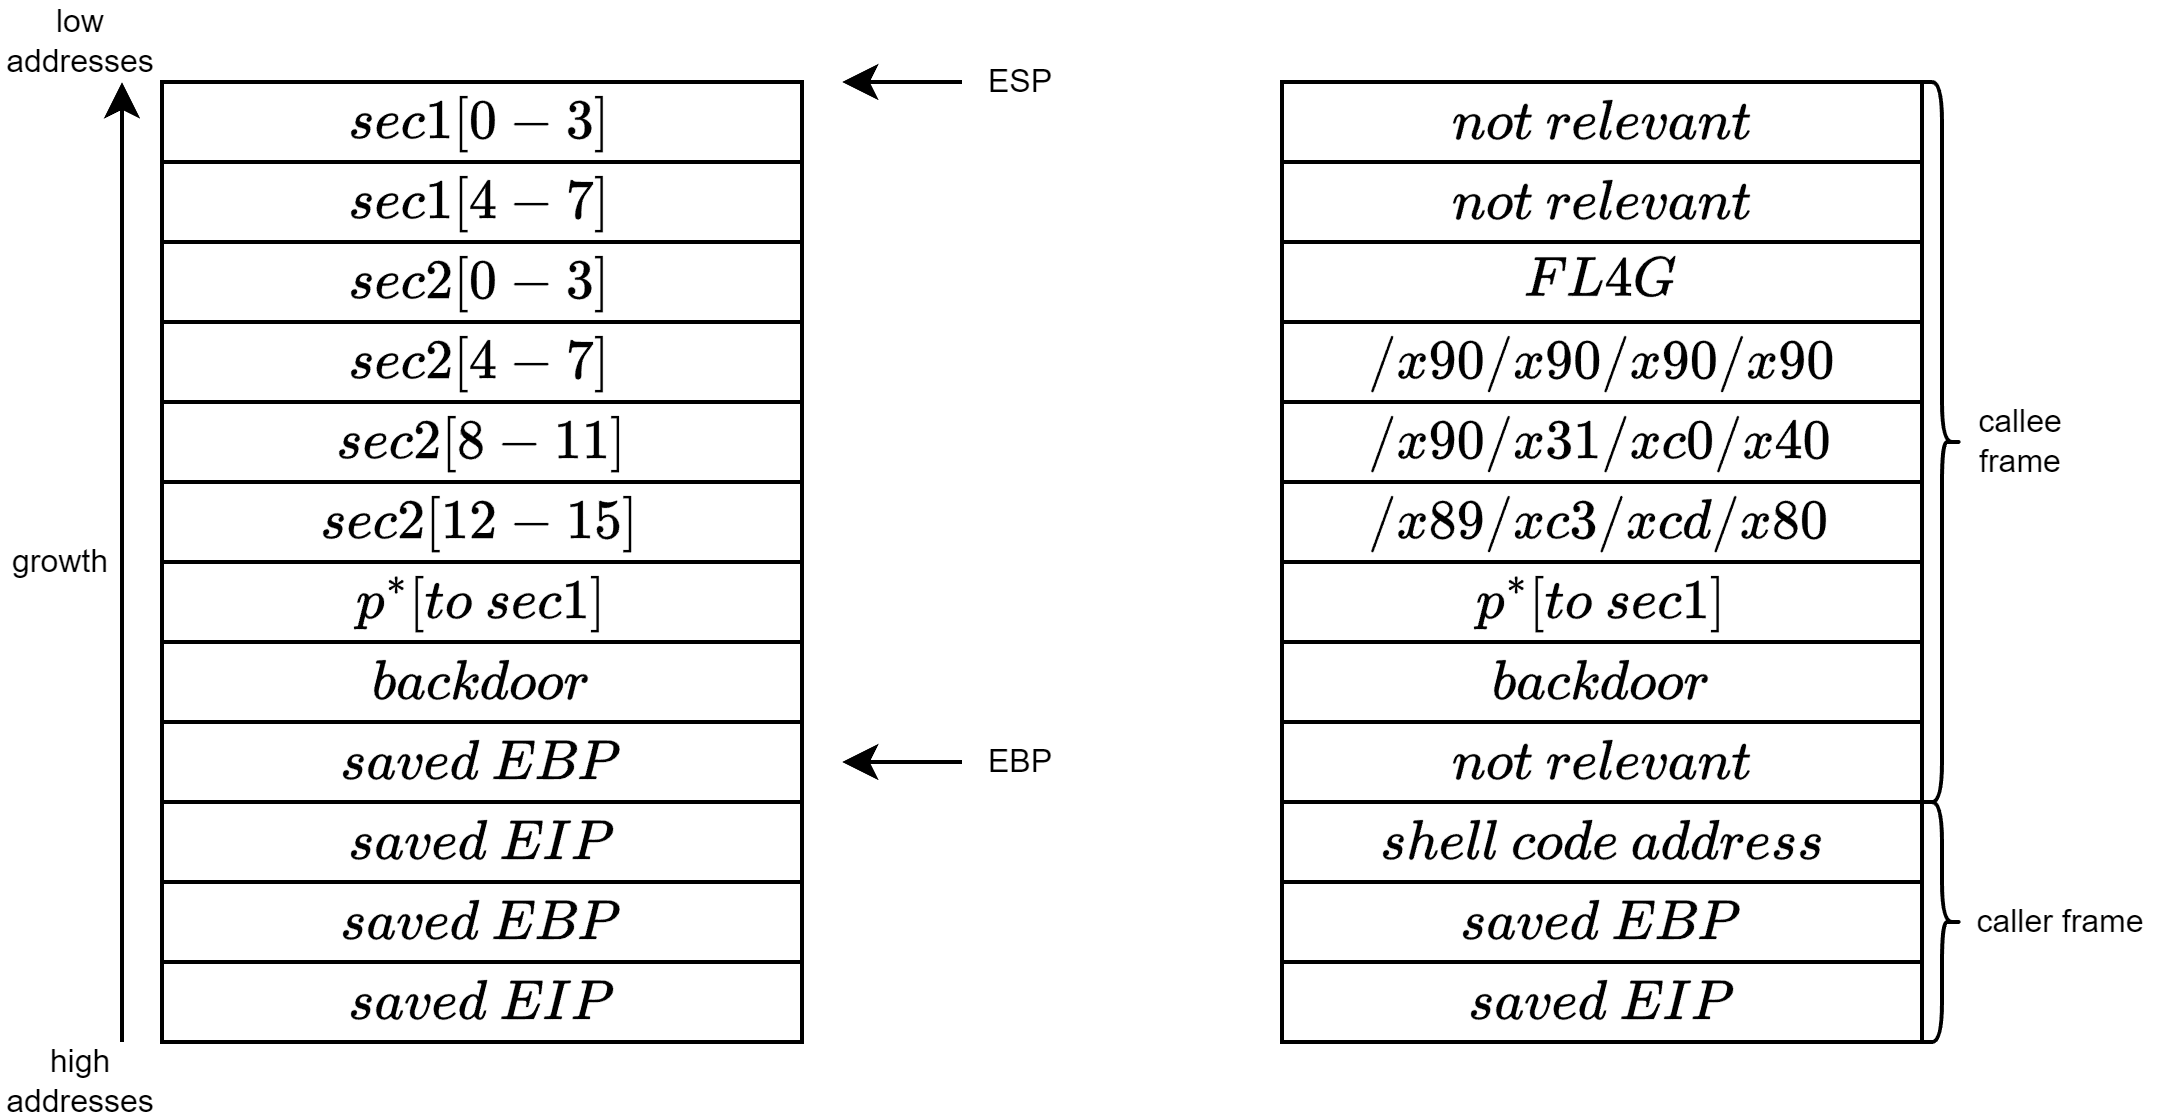
\includegraphics[width=0.8\linewidth]{images/stack11.png}
        \end{figure}
    \item The canary is inserted in the stack and checked before returning to the previous frame. 
        It detects a buffer overflow if the elements of the canary itself on the stack are changed. 
        The buffer overflow overwrite also the canary and so i will overwrite the canary and show the modification to the program that crashes. 
        A possibility to overcome this problem is to let the pointer point to the EIP, so we can directly overwrite it without touching the canary. 
    \item To exploit it, we need to write 0xf4d0e349 to 0xf b5d8.
        As 0xf4d0 > 0xe349, we don't need to swap.     
        The general format string structure is:
\begin{verbatim}
<where to write><where to write + 2>%<low value>c%<pos>$hn%<high value>c%<pos>$hn
\end{verbatim}
        \begin{itemize}
            \item Where to write = \texttt{/xd8/xb5/xf/xf}
            \item Where to write + 2 = \texttt{/xda/xb5/xf/xf}
            \item we have already written "*Decrypted*:" (12 characters) + 8 characters
            \item low value = 0xe349, so 58185 - 12 - 8 = 58165
            \item high value = 0xf7e3, so 62672 - 58185= 4487
        \end{itemize}
        Also, the displacement on the stack of the printf's argument (i.e., the buf er message) is 2, the displacement of “where to write” is 2 + 3 = 5 and the displacement of “where to write + 1” is 6.
        Complete exploit: 
\begin{verbatim}
\xd8\xb5\xff\xff\xda\xb5\xff\xff%58165c$5hn%4507c$7hn
\end{verbatim}
\end{enumerate}